
\chapter{Ubuntu Simulation}
\label{ubunutsimulation}
{}In this chapter the implementation of the conceptual model and simulation is described.
{}This simulation is validated through comparing the results of a real system to that produced by the simulation. 
{}This simulation is then used to answer some questions related to component system evolution, where the results and conclusions are discussed.

%%%What a selected component system should be like
The first choice in this implementation is the selection of the component system to study.
The selected component system should contain enough information to the resolution necessary to create a realistic configuration.
Also it should not be trivially small or simple, as the results would then be easily calculable making the simulation superfluous.

%%Why Ubuntu was selected
For these reasons the Ubuntu GNU/Linux distribution has been selected for this simulation.
This distribution contains a large and active repository of components, millions of users, and a lot of freely accessible information in order to study.
This simulation is then based on this component framework.

\section{Simulation Implementation}
There are two different aspects for the implementation of the simulation.
First the assignment of the variables in the configuration, these fall into two categories, context variables which do not change, 
and ranged variables which are changed to answer specific questions.
Also the implementation of the processes as scripts, creating a practical way of executing this simulation.

\subsection{Context Variables in the Configuration}
The context variables in the configuration are static points in the configuration that do not change across many different simulation runs.
The first context variable to be assigned is the time frame over which the simulation executes.
This leads to the assignment of the initial system invariant.
The repository function and the probability a package is selected be be installed are also invariants, and their complexity will be described.

%%%Time frame between the two releases 10.2009-10.2010, specifically from 2009,10,31 for 365 days
The time frame was selected to be over the year between the Ubuntu releases of system in 9.10 and 10.10 occurring between October 2009 to 2010.
Specifically the simulation is run from October 21st 2009 for 365 days.
The length of a year was selected as the overwhelming majority of users in our User Survey responded that their system was less than or a year old.
Ubuntu has 6 monthly releases one, in April and one in October, the syntax of the version of each release is first the year,
then the month in which it was released, e.g. 10.04 is the release in April 2010.
Therefore, this time frame occurs over an intimidate release of version 10.04 in April 2010, which allows for experimentation involving the release date.

%%%This time frame implies the initial system which is Ubuntu 10.09
The time frame start was selected to coincide with the release of a new Ubuntu version, 9.10.
This version was then selected to be used as the initial system, as if the user just installed a new Operating System onto their system.
Specifically the desktop i386 distribution was selected as it is the most popular among the users of Ubuntu.

\subsubsection{Repository function}
The repository function must return the components in the repository as a CUDF file, on any day over the course of the year.
To accomplish this the Ubuntu repository was downloaded and annotated with the times that the package was uploaded.
The mapping from Debian Package format to the CUDF (described in chapter \ref{implementation}) was then used to convert each of the downloaded packages into CUDF.
These CUDF representations where then aggregated into days they where uploaded to the repository, which can then be used to create the repository function.
Some packages are not included in the 

%%%The downloading and scraping of the ubuntu repository
The Ubuntu Repository, as with most open and free software, is freely downloadable.
It contains all the packages that have ever been in the repository with the information of when the package was added.
A web scraper was created to download all the packages, and then annotate the downloaded file with the information of when it was added to the repository.

%%%The mapping of the packages to CUDF format including the date stamp
Each package that was for the proper chipset (i386 or all), then had it's meta information from its ``control'' file extracted and converted into CUDF format.
Using the extensible syntax of CUDF we included a property ``date'', an integer type that is the time in seconds since the epoch it was added to the repository.

%%%Aggregated into dayly uploaded, then into the repository for a given day
All the CUDF files where then aggregated into the days they where added (assuming GMT dates).
These where then further combined into all the packages in a repository on a given day.
Through using these aggregated repositories a function can easily be created to return the packages on a given day.

\subsubsection{Probability a component will be selected}
%%%The probability a component will be selected
To calculate the probability a component will be selected, 
the set of packages listed in the package app-install-package is weighted with their popularity from the Ubuntu popularity contest.
The main drawback of this data is that not all packages a user may install are listed.

%%%What packages may a user select to install? We can determine this by looking at applications that are listed in the app-install-data package
There are many of the packages in a repository that a user would not directly select to install.
Most packages provide libraries, background daemons, interfaces between services; packages that are only needed through dependencies.
A user would not likely install these as they do not directly allow the user to complete tasks in the system.

The package app-install-data contains a list of applications, that are available in the repository, which the user may wish to install.
This data is used by applications like the Ubuntu Software Center to provide a mechanism for a user to find a package they may wish to install.
This comprehensive list currently\footnote{May 24th 2011} contains 2399 packages which the user may wish to install.
Some of these packages are already installed in the initial system, and some are not available in the core repository.
After filtering such packages out, the list has 2087 packages that the user can select to install from. 

%%%PopCon
The list of packages provided through the app-install-data package must still be weighted for their probability to be installed.
For this task the data set available from the Ubuntu popularity contest\footnote{http://popcon.ubuntu.com/} is used.
The Ubuntu popularity contest\footnote{http://popcon.ubuntu.com/} is an excellent, accurate and broad data-set of information of the popularity of Ubuntu packages.
Each week this automated survey is submitted by nearly two million users.
It aggregates information on what packages a user has installed and what package a user actually uses.
Through weighting the list from the app-install-data package with the number of systems that package is installed on,
the probability a package is selected to be installed can be calculated.
With the amount of information that this provides it is likely a very accurate weighting.

%%%The core problem with this list is that not all packages that can be installed are listed, i.e. experienced users may install packages that are not applications, build-essential
Although a user will more likely install packages from the app-install-data list, it is not a complete list of packages that a user may install. 
For example, more experienced users may select to install packages that are libraries or development tools, that are not listed.
The package build-essential which contains tools to build Debian packages, is not included in the list, though is regularly installed.
This is a problem that was briefly described in chapter \ref{simulation}, where different types of user are likely to install different things.
It is an extremely difficult problem to solve, and any solution will also dramatically increase the complexity of the simulation.
Therefore, this has been left out of the simulation. 

\subsection{Ranged Variables in the Configuration}
How the configuration of the simulation is altered to answer the necessary questions is through is limited to a small set of varaibles.
These variables include the criteria the resolver updates and installs packages with,
the cycle at which the users update and the probability a user will install a package.
These variables are selected as the focus of this study is on the strategy the user employs to evolve their system,
and these are somewhat under the users control.

The aspects of these variables that will be considered is the range at which they can be assigned.

\subsubsection{Criteria}
%%%What criteria will be considered
Which criteria are selected to be used by the resolver to install or update the system will effect the way the system is evolved.
The specific criteria that will be selected will be those that best suit each question. 


\subsubsection{Probability a user will Install or Update}
%%%The probability of how many components a user selects to install

%%%Never selecting anything to install is the control case
With the survey a call some logs from users where collected.

%%%We populate this field by randomly selecting from a set of real user rates.

%%%User Logs: cannot use other than Apt logs, count number of installations per day over a period of time, calculate how often they select to install
Resolvers often keep logs of their activities, for reporting and bug tracking purposes.
When distributing the user survey their logs where asked for as this may help with the definition of this field.

%%%We can either use these values to bootstrap to our simulation, or we can define our own values to stress test.

\subsection{Scripts of Processes}
The processes described in chapter \ref{simulation} have been implemented using a set of BASH and Python scripts.
First these scripts generate a user action files, which is a store for user actions so that they can be reused with different configurations.
These are then used with the criteria for installation and updating by a script to generate CUDF problems and execute the simulation.

\subsubsection{Generate User Script}
%%%The process used to generate files
The generate user script is an implementation of the process described in figure \ref{generateuser}, it takes in the configuration and generates a set of tuples, which are stored in the user file format.
An example of a user file is shown in figure \ref{userfile}.

%%%The User file
\begin{figure}[htp]
\begin{center}
1258110000.0;;;update
1258196400.0;;;update
1258282800.0;install:vinagre;;update
1258369200.0;install:compiz-core;keep:vinagre;update
1258455600.0;;keep:vinagre,compiz-core;update
1258542000.0;install:gdebi;keep:vinagre,compiz-core;update
  \caption[User File example]{An example of a User file}
  \label{userfile}
\end{center}
\end{figure}

This user file follows the grammar ``time;[install:PACKAGE[,PACKAGE]*]?;[keep:PACKAGE[,PACKAGE]*]?;[update]?''.
This directly maps to the user action tuple with a time variable, an install action, a keep action, and an update action separated by a delimiter of ``;''.

%%%Pratical differences between the pseudo code and real script, creating multiple users per configuration. And inputting multiple User cycles, and User install distribution to create 
The practical use of this algorithm differs in a few aspects, that should be discussed.
Firstly, given the random process introduced by probabilities in the configuration e.g. user package installation,
a single generated user may not be representative of the entire group, so multiple users for the same configuration can be generated in the actual script.
This allows the input of multiple values from the configuration variables update probability, user install distribution.

The generation of multiple user action files has two benefits, it lowers the loading and processing of some of the data, notably package distributions, which can be intensive on computer resources.
Also it makes the script more usable as generating many different user action files individually can be a time consuming task.

The representation of the configuration variables for the user install distribution and the probability a package is installed have their own file formats.
These are presented in figures \ref{userprob} and \ref{packageprob}.

In figure \ref{userprob} is an example of the file describing the probability disturbance of a users likely hood to install a number of packages.
Each line represents a user, each list of real numbers is a users probability distribution separated by the delimiter ``,''.
The first line then means that a user has a 75.5\% chance of installing 0 packages, a 17.5\% chance of installing 1 package and a 5\% chance of installing 2 packages per day.

\begin{figure}[htp]
\begin{center}
75.5, 17.5, 5.0
73.0, 18.0, 6.0, 1.0
54.0, 34.0, 9.0, 2.0
\caption[Install Distribution Example File]{An example of a users installation distributions}
\label{userprob}
\end{center}
\end{figure}

In figure \ref{packageprob} the file is laid out as a list of lines, each line is package name, then an integer separated by a comma.
The integer is the weight which represents the likelihood the package will be selected to be installed.
To convert this weight into the necessary probability, the individual package weight is divided by the the sum of all package weights. 

\begin{figure}[htp]
\begin{center}
gstreamer0.10-plugins-ugly,1398598
gstreamer0.10-ffmpeg,1389240
scim,1273746
pidgin,1185436
gstreamer0.10-plugins-bad,1147125
notification-daemon,1115926
\caption[Weighted Package File Example]{An example of a Weighted Package file }
\label{packageprob}
\end{center}
\end{figure}

\subsubsection{Execute Simulation}
The scripts to generate the CUDF problem and execute the simulation, described in the chapter \ref{simulation}, 
are used to take a set of user interactions and criteria for update and install and simulate a solvers evolution.
These process are implemented in the scripts based directly off of their described processes. 
However, some practical changes were made in order to decrease the resources consumed when the scripts are executed and make the scripts easier to use.

%%%Executing multiple users in a row
As many different sets of user actions require to be generated, executing one set at a time is a tedious task.
Using multiple user files to execute the run simulation algorithm in series increased the usability of the script.
This is simply done by iterating over a set of user files inputting one at a time into the algorithm. 

%%%The addition of the timeout
One additional input is required, the timeout variable which allows the system to stop the process of the resolver and return the best solution currently found.
This timeout variable is simply an integer representing the number of seconds that the solver is allowed to run for.
The resulting impact of the time out remains to be seen, having it is just to ensure that the simulation operates within a upper bound of time.
It may effect certain criteria and strategies more than others, this may have an impact on the results and the decision between different strategies.

\subsection{Verification}
%%%How we tested and made sure that the output was what it should be
The way in which this simulation is implemented is abstracted from the configuration that is provided.
This means that creating a ``mock'' configuration in order to be tested is simple.
This testing was simplified because of the separation between the processes of generating the user actions, generating the CUDF problem, and executing the simulation.
The resolver was tested and thoroughly verified to work through the MISC, and its individual criteria where tested as well for correctness.

%%%Generate User Actions
The generation of the user actions was tested by first inputting various configuration and taking what actions where generated and ensuring that they conformed to the input.
For instance, by stating a user will update 50\% of the time, creating a set of user actions and ensuring that it is correct, it can be assumed that function is correct.
This was also done for the install distribution and the weighted packages input.

%%%Generate CUDF
This testing of the generation of the CUDF problem was tested through giving the script a configuration and user action, and ensuring that it generated the problem correctly. 
For instance, giving the script a user action to install package ``a'' and keep package ``b'', then looking at the output problem for correctness.

%%%Execute Simulation 
The testing of the execute simulation script was done through extensively logging the process and ensuring the individual functions where correct.
As this script is a simple iteration the main task is to ensure that all the functions occur in the proper order and that no exceptions occur.
This can be done through passing it various inputs and ensuring that they are properly processed.
The individual functions of \verb+FAIL+ and \verb+executeSolver+ can be verified separately.
These can have various inputs and checked for correct output.

%%%The resolver validation though MISC
The resolver is the most complex code in this simulation, the verification of this has been described in chapter \ref{implementation}.
This was done through testing and the entrance into two MISC competitions, which ensured third party verification of the core resolver.

%%%The criteria validated through checking for correct constraints and estimates
This process verified the resolvers implementation and some of the criteria defined.
However, there are many criteria used in this simulation that where not verified through this process.
Many of the criteria used in this simulation where verified through firstly ensuring the correct constraints where being generated, 
and ensuring the output solution conforms to the constraints.
They where adjusted for speed through testing them against many of the CUDF problem from the MISC.

\section{Simulation Validation}
The validation of the implementation of the simulation is an important step in the use of this simulation.
It is done in an attempt to shows the similarities and the differences to reality.
As a simulation is only an approximation it will never be identical to a real system, the hope is that it is different by a tolerable error. 

This validation is accomplished though looking at the results outputted from the simulation.
This is done in two ways, firstly by taking the results and ensuring that it conforms to what we believe the system should act like.
The second way is through comparing these results with the output of the actual system.

%%%Face Validation
Face validation is the process by which output of the simulation is given to experts in order to find if it behaves as they believe it should.
The core output from this simulation is the resulting systems created during execution of the simulation.
Looking at this output alone is difficult to state that it is correct, only that it looks correct.

\subsection{Controlled Validation}
%%%Controlled Environment
To attempt to validate this simulation a controlled environment was set up. 
A computer had a recent Ubuntu version installed, and each day a script was executed that updated the system, and saved the repository and the system state.
This information was then used to simulate this process and the results analyised for simlarity.
%TODO  

\subsection{Validation against User Log}
%%%Real User Log
To further validate this simulation, results configuration was used.
This is where the output of a real system is compared to those created from the simulation.
A user log that is from the Ubuntu distribution is used as the output from a real system. 
From this log a configuration is generated; the update probability, the install distribution and the range of dates are extracted from the log.
The update and install criteria are that used by the APT application, and the rest are the default contexts.  

The results of the simulation given this configuration where then compared to see if the changes made to the simulated system where similar to that of the real system.
%TODO

\section{Questions}
This simulation has been defined and implemented in order to answer questions about component system evolution.
Defining the scope of these question is important, to stop the snowballing effect where getting answers can lead to more questions. 

The scope is defined through the core question of this research:

``What effect does using component resolution with different strategies have on system evolution?''.

This question has been broken up into three sub-questions,
\begin{itemize}
  \item Question 1 looks at strategies for updating
  \item Question 2 looks at different strategies for installing
  \item Question 3 looks at combining of installing and updating strategies
\end{itemize}

In this section these questions are broken into specific questions which are attempted to be answered though using our simulation.

\subsection{Question 1}
The most significant action for the evolution of a users system is through requesting to update its components.
This action can effect all components in the system, and can cause major changes in the way in a systems structure.
The strategy the user employs to update, involves how often they update, and what criteria they optimise their resolver for when updating.
As the installation is ignored in these questions, the install probability is set to 0 in the configuration.


\subsection{What are the effects of the extreme update strategies?}
%%%We answer this to find the range in which users can select their strategies
As described in chapter \ref{strategies}, the two main user sterotypes are that of the conservative user, who never wants to change their system,
and the progressive user, who wants to be most up to date.
These two extremes of this strategy are first measured to find the range in which all questions can be answered.

An extreme conservative user never wants to change their system, therefore their update strategy is to never update.
This will mean that there system will never update, and how fast they become out of date as this is what they are sacrificing is of interest.
This means that the criteria used for updating is unnecessary as it is never updated, and the user update probability will be 0.

On the other hand, an extreme progressive user will update every day with criteria where being up to date is the highest importance.
This will make this system change as much as necessary in order to have the newest components.
Specifically, the criteria that is used will be ``-uptodatedistance,-removed,-new'', and the user update probability will be 1.

\subsubsection{Results and Analysis}
The results are presented here.

\subsubsection{Conclusions}
These users represent only the most extreme users, and not the typical users strategy.
However, all other strategies exist between these two giving us a range of exploration in further questions.

\subsection{What are the effects of strategies that current users employed?}
%%%What is currently done in order to update a system
Through selecting a range of user submitted logs and extracting their update probabilities, a ``real'' users actions can be predicted.
These actions can then be simulated using different criteria from current resolvers.

The two resolvers that are being looked at are APT, the default Debian and Ubuntu resolver, and Eclipse P2, the Eclipse provisioning system.
As described in chapter \ref{strategies} the criteria for APT is ``-removed,-new,-uptodatedistance'', and for P2 it is ``-uptodatedistance,-removed,-new''.
The difference between these two resolvers is that APT is a conservative resolver, where Eclipse P2 is more progressive. 

Using these defined configurations 10 runs for each of 5 selected users where executed. 
These users where selected to represent a broad range of different update probabilities, and the amount of runs as different user probabilities will create different user actions.

\subsubsection{Results}
The results from this simulation are presented here:

The results when compared to the two extreme users presented in the previous question:

\subsubsection{Conclusion}
These results are interesting to note for two reasons. 
Firstly the difference over the time period when updating with either APT or Eclipse P2 is shown to be\ldots

When compared to the extreme users, there is a significant amount of area that the conservative.
How conservative users change their systems could be 

\subsection{What effect does a users update frequency have?}
%%%Why a user selects to upgrade at their update probability
A user will select to upgrade their system in order to increase the functionality of their system and to reduce risk of bugs being introduced.
These benefits are weighted against against the risk that it causes on their system due to the necessary change, to define the probability a user will upgrade on a given day.

%%%We have already explored the extremems and some real user probabilities, now we explore this as a range
The extremes of the users probability to upgrade, from updating every day to never upgrading, have been explored.
Also, some users have been simulated to see the effect on their update probabilities extracted from the submitted user logs.
Here, the update probability simulated over a range of possibilities, to find the relationship between it and the resulting systems probabilities.
For instance, what is the difference between a user who updates every day to one that updates half as much?

Specifically, the update probability is selected to be $[0,0.1,0.2,0.3,0.4,0.5,0.6,0.7,0.8,0.9,1]$,
selected as they cover the range of all update probabilities.  
The criteria will be the conservative ``-removed,-new,-uptodatedistance'', and progressive ``-uptodatedistance,-removed,-new''.
Each strategy (expect where the update probability is 1 or 0), will be executed 10 times to give a range of possible outcomes.

\subsubsection{Results}
The results are presented

\subsubsection{Conclusion}
The difference between updating 1 and .5 is insignificant. 

\subsection{What are the effects of only installing stable components?}
%%%We noticed something interesting
An interesting relationship was noticed when looking at the release cycles of different components;
components will often release a versions very close together then have long periods of not releasing.

%%%It might be caused by this
This effect may be caused by users of the package updating to the newly released verion, 
finding and posting bug report to the maintatin, who then quickly fixes the bug and releases a new versions to resolve the issue.
 
%%%Here is a real example of this happening
An example of this described situation is show in figures \ref{apachelog} and \ref{apachebug}.

\begin{figure}[htp]
\begin{center}
\begin{alltt}
apache2 (2.2.20-1) unstable; urgency=low

  * New upstream release.
  * Fix some regressions related to Range requests caused by the CVE-2011-3192
    fix. Closes: #639825
\ldots

 -- Stefan Fritsch <sf@debian.org>  Sun, 04 Sep 2011 21:50:22 +0200

apache2 (2.2.19-2) unstable; urgency=high

\ldots

 -- Stefan Fritsch <sf@debian.org>  Mon, 29 Aug 2011 17:08:17 +0200
\end{alltt}
\caption[Apache Changelog]{An extract from the apache changelog located on http://changelogs.ubuntu.com/}
\label{apachelog}
\end{center}
\end{figure}

\begin{figure}[htp]
\begin{center}
\begin{alltt}

Reported by: Takis Issaris <takis.issaris@uhasselt.be>
Date: Tue, 30 Aug 2011 16:09:01 UTC
Severity: important
Found in versions 2.2.9-10+lenny10, 2.2.16-6+squeeze2, apache2/2.2.19-2

\ldots

Package: apache2.2-common
Version: 2.2.9-10+lenny10

Yesterday evenings update broke our Apache server setup,
\ldots
\end{alltt}
\caption[Apache Bug Report]{Extract from the bug report \#639825, filed with Debian}
\label{apachebug}
\end{center}
\end{figure}

A summary of these evenets are:
\begin{enumerate}
  \item Apache developer Stefan Fritsch released a new version of their server, apache2/2.2.19-2, on 29 Aug 2011
  \item Takis Issaris upgraded to this version which broke their system on 29 Aug 2011
  \item Takis Issaris submits a bug report on 30 Aug 2011, where he and Stefan Fritsch discuss the causes
  \item On 04 Sep 2011 Stefan Fritsch releases a new version 2.2.20-1 that fixes this bug
\end{enumerate}



\subsubsection{Measuring the Effect}
By calculating the difference in days between each version of all components in the repository, 
over the dates of the simulation how often this situation occurs, where packages are quickly updated, can be measured.
In figure \ref{comeponentversionreleases} a graph is presented measuring the time difference between version releases.
 
\begin{figure}[htp]
\begin{center}
  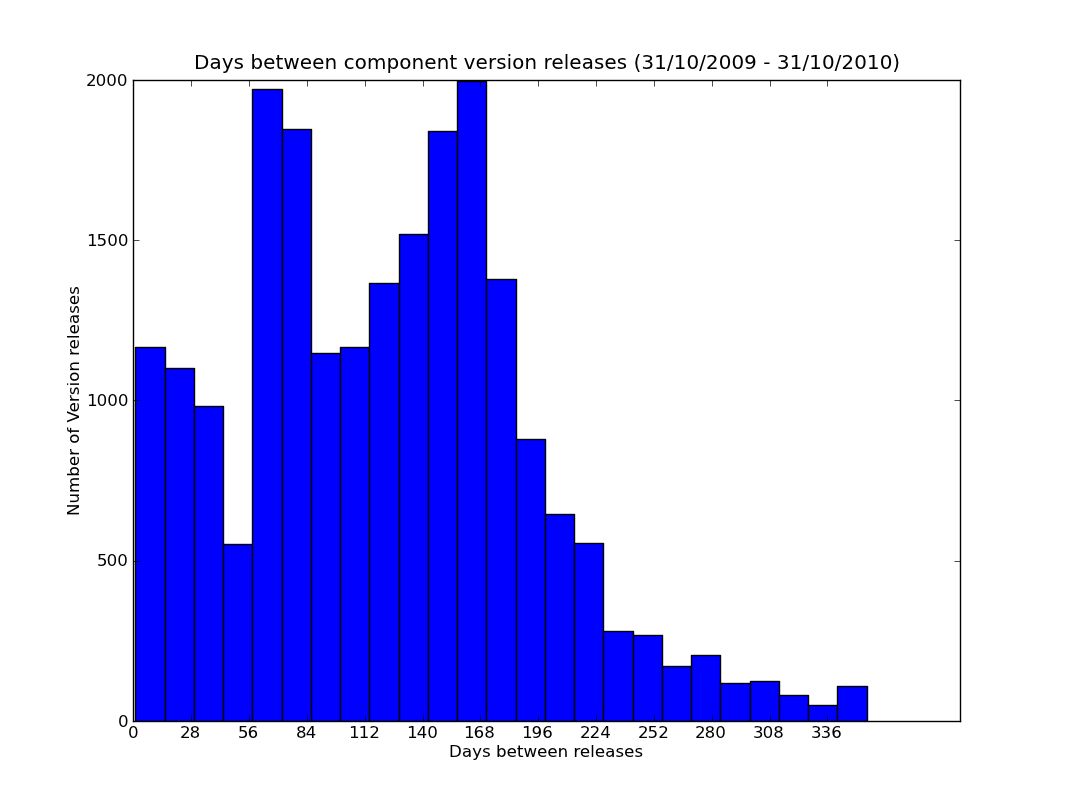
\includegraphics[width=\textwidth]{ubuntusimulationpics/versionreleasedistribution}
  \caption[labelInTOC]{Distribution of the releases of component versions between 31/10/2009 - 31/10/2010}
  \label{comeponentversionreleases}
\end{center}
\end{figure}

There are two points on this graph are noteworthy, firstly there is a large amount of components that release after 3 and 6 months.
Secondly there is a smaller but significant amount of components that have been released less than a month after the previous release.

The release of components after 3 or 6 month is probably due to the 6 monthly release cycle of Ubuntu.
Where individual components will release new versions for each Ubuntu release for it to be included.

\subsubsection{Effects of these releases}
%%%If this happens a lot, then these effects will happen
If this kind of release happens frequently to components in a repository, it causes much more change for a progressive user,
and standard strategies leave both conservative and progressive users vulnerable to the possible bug.

%%%A progressive user will experience a great deal more change with little benefit
The main effect of this kind of release causes to a progressive user is their system will go through more changes with little benefit.
As a progressive user will update frequently, it means they may upgrade to each release of a component.
As the time between the releases are so close to each other this only introduces more risk, and has little benefit for the system.

%%%Both types of users are vulnerable if the bug effects them
Another problem caused by this type of release is that if the bug effects the system, conservative users as well as progressive users are vulnerable.
Conservative users, although they update less frequently do update sometimes.
The time in which they update could be between one of these releases and then the bug can be introduced into their system, 
causing them to update once more, maybe introducing another bug.


\subsubsection{Criteria}   
The effects caused by these components that release soon after, i.e. within a month, of a previous release can be mitigated by taking into account when a component was released.
This criteria will then wait a certain amount of time once a package has been released, ensuring that no more releases are coming.
This idea is called ``Stable Version'', the main parameter that is required is the time in which to wait for a package to become stable.

This stable release criteria is defined as a hard constraint that can be added to a users update criteria.
%%%TODO

To test this criteria, to see if it reduces the effects of a set of user values is selected from the logs and extremes to build sets of user actions.
Through altering our progressive and conservative criteria to include the stable version criteria a range of values for the parameter of stable version is tested and measured for performance.
The criteria are altered to ``-stableversion(N),-removed,-new,-uptodatedistance'' and ``-stableversion(N),-uptodatedistance,-removed,-new'' where N is a number from a selected range.

\subsubsection{Results}
Compare against extreme and normal update distances.

\subsubsection{Conclusions}
The addition of the stable version criteria is shown to improve both the conservative and progressive user criteria.

It also shows that updating daily with a large stable version parameter is more conservative with better metrics than updating less frequently with no parameter.

\subsection{Should the system be updated on or after a release?}
A release of a component system is a milestone in the systems development.
It involves the cooperation of many parties, inclusing the component systems managers, and the component developers.
This usually has many formal aspects to it, in Ubuntu there is an official schedule which is followed, an example shown in figure \ref{ubuntuSchedule}

\begin{figure}[htp]
\begin{center}
  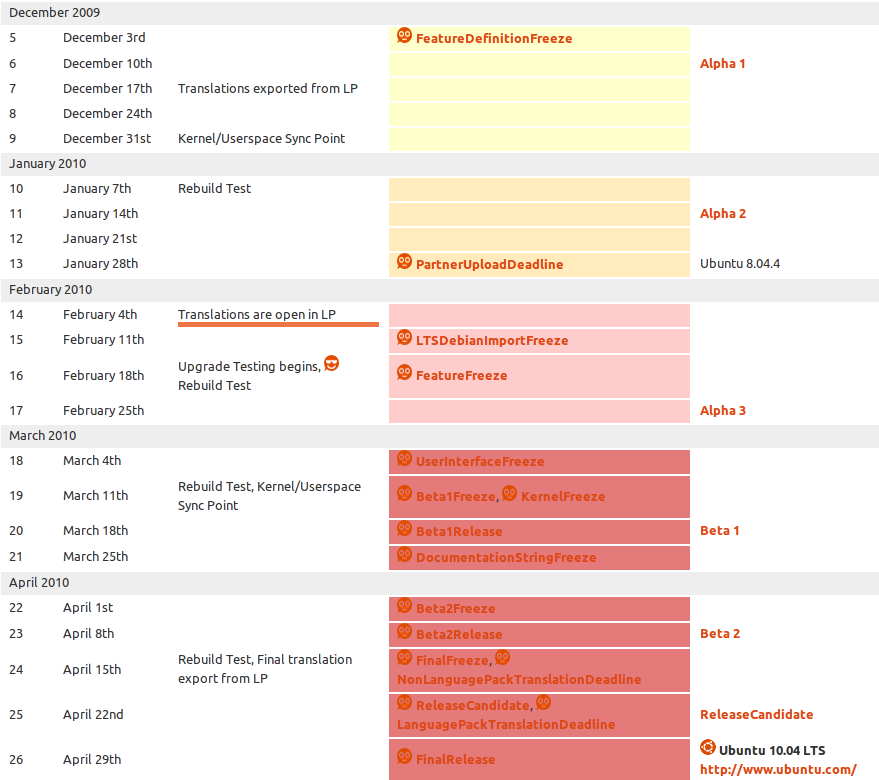
\includegraphics[width=\textwidth]{ubuntusimulationpics/ubunturelease}
  \caption[labelInTOC]{The Ubuntu release schedule from https://wiki.ubuntu.com/LucidReleaseSchedule}
  \label{ubuntuSchedule}
\end{center}
\end{figure}

These releases have an effect on the amount of packages aded to a repository, as can be seen in figure \ref{}

\begin{figure}[htp]
\begin{center}
  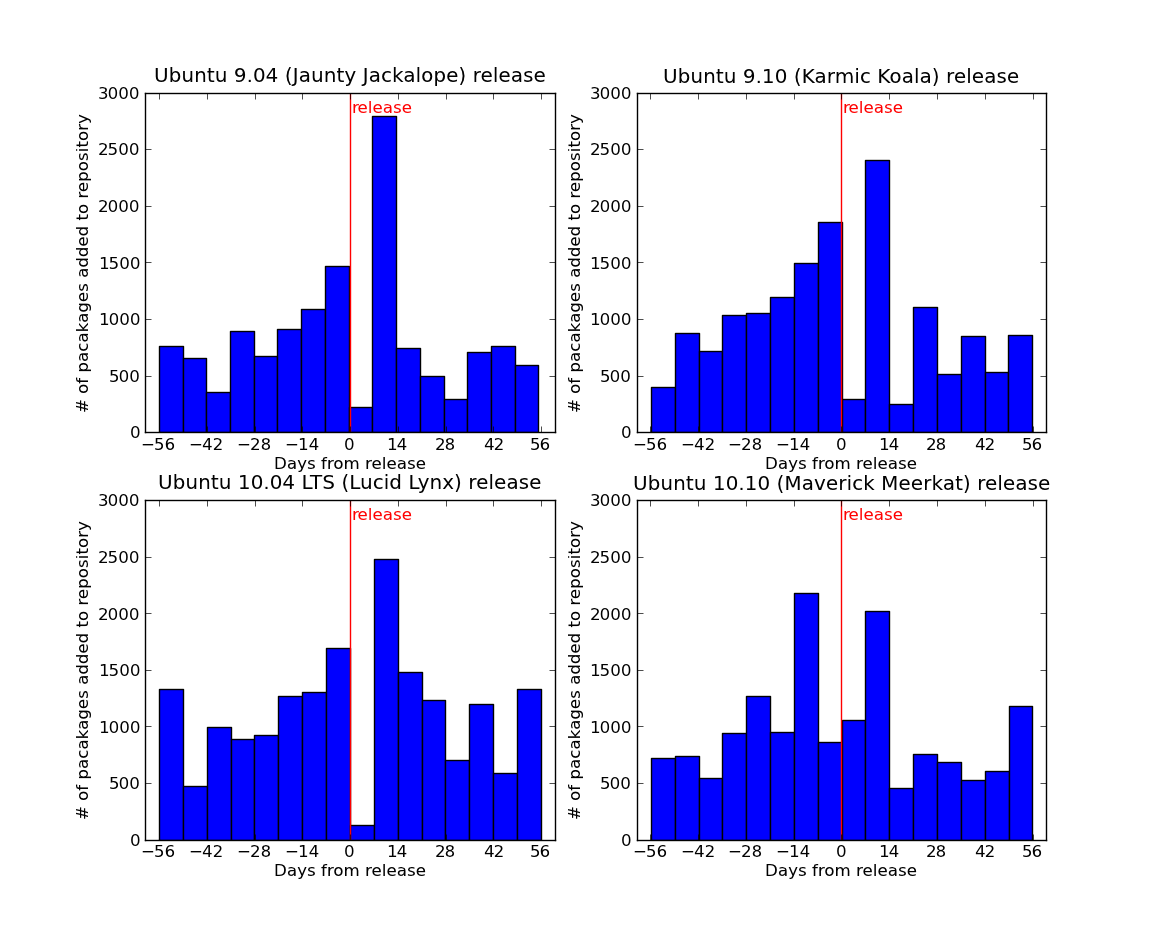
\includegraphics[width=\textwidth]{ubuntusimulationpics/releasedatepacakges}
  \caption[labelInTOC]{The amount of packages added to the repository in relation to the Ubuntu releases}
  \label{ubuntuSchedule}
\end{center}
\end{figure}


\subsubsection{Results}

\subsection{What is the effect of either progressivly or conservativly updating for reccommends as well?}


\section{Summary}
%%%A list of the answers gained from the questions
